\chapter{Implementacja}\label{chap:implementacja}

Rozdział opisuje platformę eksperymentalną zbudowaną na potrzeby porównania
sześciu architektur agentowych w~zadaniu odpowiadania na pytania dotyczące
polskich dokumentów ubezpieczeniowych. W~rozdziale omówiono stos
technologiczny, podział kodu na moduły, komponenty współdzielone przez
wszystkie warianty, implementację promptów, narzędzi agentowych i~grafów
sterowania, potok przetwarzania dokumentów, infrastrukturę ewaluacyjną oraz
wybrane decyzje inżynieryjne.

Kompletny kod źródłowy systemu, w~tym konfiguracja środowiska i~skrypty
eksperymentów, udostępniono w~publicznym repozytorium GitHub pod adresem
\url{https://github.com/mchojna/master-thesis-pjatk}.

Implementację oparto na założeniu metodologicznym, w~którym architektury różnią
się wyłącznie sposobem sterowania przebiegiem zadania. Dokumenty, indeks
wektorowy, zestaw narzędzi, konfiguracja modeli, format odpowiedzi i~procedura
ewaluacji są wspólne dla wszystkich wariantów. Podejście to determinuje
strukturę kodu, wymuszając wyraźną granicę między warstwą sterowania a~warstwą
operacyjną.

\section{Stos technologiczny}\label{sec:stos-technologiczny}

System zaimplementowano w~języku \texttt{Python} w~wersji 3.13. Warstwę
orkiestracji oparto na bibliotece \texttt{LangGraph}, umożliwiającej
definiowanie grafów stanowych z~węzłami asynchronicznymi, krawędziami
warunkowymi i~kontrolowanymi pętlami. Właściwości te są niezbędne do
odwzorowania różnic między topologiami. Dostęp do modeli językowych i~modelu
osadzeń zapewnia \texttt{LangChain} wraz z~pakietem \texttt{langchain-openai}.
Fragmenty dokumentów przechowywane są w~bazie wektorowej~\texttt{Qdrant},
a~warstwa ewaluacji i~rejestracji przebiegów korzysta z~\texttt{Arize Phoenix},
\texttt{PostgreSQL} oraz \texttt{OpenTelemetry}.

Tabela~\ref{tab:stos-technologiczny} zestawia komponenty stosu wraz z~wersjami
i~rolami w~systemie.

\begin{table}[H]
  \caption{Stos technologiczny}\label{tab:stos-technologiczny}
  \centering
  \small
  \begin{tabularx}{\textwidth}{@{} l l l L @{}}
    \toprule
    \textbf{Warstwa}
    & \textbf{Komponent}
    & \textbf{Wersja}
    & \textbf{Rola}                                                              \\
    \midrule
    Środowisko uruchomieniowe
    & \texttt{Python}                                           & \(\geq\)3.13
    & Język implementacji                                                        \\
    \addlinespace
    Orkiestracja agentów
    & \texttt{LangGraph}                                        & \(\geq\)0.2.0
    & Grafy stanowe architektur agentowych                                       \\
    \addlinespace
    Warstwa modeli językowych
    & \texttt{LangChain}, \texttt{langchain-openai}             & \(\geq\)1.2.10
    & Klienty modeli i~osadzeń                                                   \\
    & \texttt{OpenAI API}                                       & \(\geq\)2.21.0
    & Wywołania \texttt{gpt-5}, \texttt{text-embedding-3-large}                  \\
    & \texttt{Pydantic}                                         & \(\geq\)2.12.5
    & Schematy wyjść strukturalnych                                              \\
    \addlinespace
    Warstwa wyszukiwania
    & \texttt{Qdrant}                                           & 1.15
    & Baza wektorowa i~filtry metadanych                                         \\
    \addlinespace
    Warstwa ewaluacji
    & \texttt{Arize Phoenix}                                    & 13
    & Ewaluatory LLM-as-a-judge i~panel śledzenia                                \\
    & \texttt{PostgreSQL}                                       & 14
    & Baza operacyjna usługi \texttt{Phoenix}                                    \\
    \addlinespace
    Przetwarzanie dokumentów
    & \texttt{pypdfium2}, \texttt{Pillow}                       & \(\geq\)5.4.0
    & Renderowanie stron PDF do obrazów PNG                                      \\
    & \texttt{langchain-text-splitters}                         & \(\geq\)1.1.0
    & Fragmentacja Markdown po nagłówkach i~rekurencyjna                         \\
    \addlinespace
    Infrastruktura pomocnicza
    & \texttt{tenacity}, \texttt{structlog}                     & \(\geq\)9.1.4
    & Ponowienia wywołań i~logowanie strukturalne                                \\
    \bottomrule
  \end{tabularx}
  \zrodlo{opracowanie własne na podstawie pliku \texttt{pyproject.toml}}
\end{table}

W~systemie wyróżniono trzy klasy artefaktów. Danymi wejściowymi są pliki PDF
z~dokumentami OWU i~IPID oraz plik CSV z~pytaniami testowymi. Artefaktami
pośrednimi są pliki Markdown powstałe po ekstrakcji i~kolekcja \texttt{Qdrant}.
Artefaktami końcowymi są odpowiedzi agentów, metadane wykonania oraz pliki
ewaluacyjne. Tabela~\ref{tab:artefakty-systemu} zestawia wszystkie klasy
artefaktów z~ich lokalizacją i~zastosowaniem.

\begin{table}[H]
  \caption{Artefakty systemu}\label{tab:artefakty-systemu}
  \centering
  \small
  \begin{tabularx}{\textwidth}{@{} l L L @{}}
    \toprule
    \textbf{Etap}
    & \textbf{Artefakt}
    & \textbf{Zastosowanie}                                              \\
    \midrule
    \multirow{2}{*}{Wejście}
    & \texttt{data/documents/raw\_documents}
    & Surowe dokumenty OWU i~IPID w~formacie PDF                         \\
    & \texttt{data/evaluation/questions/*.csv}
    & Pytania, odpowiedzi referencyjne i~metadane próbek                 \\
    \addlinespace
    \multirow{3}{*}{Pośredni}
    & \texttt{data/documents/extracted\_documents}
    & Dokumenty po ekstrakcji do Markdown                                \\
    & \texttt{data/documents/insurance\_documents}
    & Kolekcja \texttt{Qdrant} z~wektorami i~metadanymi fragmentów       \\
    & \texttt{data/diagrams}
    & Diagramy architektur generowane z~definicji \texttt{Mermaid}       \\
    \addlinespace
    \multirow{2}{*}{Wyjście}
    & \texttt{data/evaluation/results/runner\_results\_*.jsonl/csv/json}
    & Surowe odpowiedzi, cytowania i~metadane wykonania                  \\
    & \texttt{data/evaluation/results/overall\_*\_*.csv}
    & Artefakty ewaluacji odpowiedzi i~trafności dokumentów              \\
    \bottomrule
  \end{tabularx}
  \zrodlo{opracowanie własne}
\end{table}

\section{Architektura modułowa systemu}\label{sec:architektura-modulowa-systemu}

Główna implementacja systemu mieści się w~module \texttt{sources} i~dzieli się
na sześć warstw: konfigurację, architektury agentowe, narzędzia, potok
dokumentów, wykonanie eksperymentu oraz narzędzia pomocnicze. Podział ten
ogranicza zależności między komponentami -- wymiana jednej architektury nie
wymaga modyfikacji narzędzi wyszukiwania, syntezy ani ewaluacji.

Istotny podział wprowadzono między katalogami \texttt{agents} i~\texttt{tools}.
Pierwszy z~nich zawiera wyłącznie logikę sterowania: kolejność węzłów,
krawędzie warunkowe, pętle i~warunki zakończenia. Drugi z~kolei zawiera
operacje dziedzinowe wykonywane przez wszystkie architektury: parsowanie
pytania, przepisywanie zapytania, wyszukiwanie, selekcję dowodów, cytowania,
dobór promptu i~syntezę odpowiedzi. Żadna z~architektur nie implementuje
własnej logiki wyszukiwania ani generowania odpowiedzi.

Zależności między warstwami przedstawiono na rysunku~\ref{fig:warstwy-systemu},
a~odpowiedzialności poszczególnych modułów opisano
w~tabeli~\ref{tab:moduly-systemu}.

\begin{figure}[H]
  \caption{Warstwy systemu}\label{fig:warstwy-systemu}
  \centering
  \begin{adjustbox}{max width=0.96\textwidth}
    \begin{tikzpicture}[
        block/.style={rectangle, draw, rounded corners=4pt,
          minimum height=2.5cm, text width=5.5cm,
        align=center, font=\footnotesize},
      ]
      \node[block, fill=violet!8, draw=violet!45] at (0, 0)
      {\textbf{\texttt{runner / evaluator / observer}}\\
      uruchomienia, ewaluacja, śledzenie};

      \node[block, fill=gray!10, draw=gray!45] at (6.5, 0)
      {\textbf{\texttt{agents}}\\
      sześć grafów \texttt{LangGraph} i~fabryka architektur};

      \node[block, fill=violet!5, draw=violet!30] at (13, 0)
      {\textbf{\texttt{tools}}\\
      wspólny rejestr ośmiu narzędzi agentowych};

      \node[block, fill=teal!6, draw=teal!35] at (0, -3.5)
      {\textbf{\texttt{extractor / chunker / vectorstore}}\\
      przygotowanie Markdown, fragmentów i~kolekcji \texttt{Qdrant}};

      \node[block, fill=teal!7, draw=teal!45] at (6.5, -3.5)
      {\textbf{\texttt{config}}\\
      ustawienia, prompty, klienty};

      \node[block, fill=teal!7, draw=teal!45] at (13, -3.5)
      {\textbf{\texttt{utilities}}\\
      metryki, diagramy};

    \end{tikzpicture}
  \end{adjustbox}
  \zrodlo{opracowanie własne}
\end{figure}

\begin{table}[H]
  \caption{Moduły systemu}\label{tab:moduly-systemu}
  \centering
  \small
  \begin{tabularx}{\textwidth}{@{} l L L @{}}
    \toprule
    \textbf{Moduł}
    & \textbf{Zakres}
    & \textbf{Główne pliki}                                     \\
    \midrule
    Konfiguracja
    & Konfiguracja ścieżek, modeli, \texttt{Qdrant},
    ewaluacji i~promptów
    & \texttt{app.py}, \texttt{graph.py}, \texttt{prompts.py}   \\
    Agenty
    & Implementacje sześciu topologii i~wspólny stan
    & \texttt{state.py}, \texttt{factory.py}, pliki architektur \\
    Narzędzia
    & Rejestr i~implementacja narzędzi agentowych
    & osiem modułów narzędziowych.                              \\
    Potok dokumentów
    & Ekstrakcja PDF, fragmentacja i~indeksowanie
    & \texttt{extractor.py}, \texttt{chuncker.py},
    \texttt{vectorstore.py}                                      \\
    Wykonanie
    & Uruchamianie macierzy pytań i~architektur
    & \texttt{runner.py}                                        \\
    Ewaluacja
    & Przygotowanie danych dla \texttt{Phoenix} i~zapis metryk
    & \texttt{evaluator.py}, \texttt{observer.py}               \\
    Pomocnicze
    & Śledzenie kosztów, tokenów i~renderowanie diagramów
    & \texttt{tracker.py},
    \texttt{drawer.py}                                           \\
    Notatniki
    & Sterowany przebieg przygotowania indeksu,
    uruchomień i~ewaluacji
    & \texttt{NB\_00} -- \texttt{NB\_04}                        \\
    \bottomrule
  \end{tabularx}
  \zrodlo{opracowanie własne}
\end{table}

\section{Elementy architektury współdzielone}\label{sec:elementy-architektury-wspoldzielone}

Komponenty współdzielone stanowią podstawę wszystkich architektur. Obejmują
wspólny obiekt stanu, konfigurację uruchomieniową, zamknięte schematy wyjść
strukturalnych, rejestr narzędzi oraz fabrykę grafów.
\subsection{Stan grafu}\label{subsec:stan-grafu}

Węzły grafów komunikują się za pomocą typowanego słownika
\texttt{ExperimentState}, zdefiniowanego w~\texttt{sources/agents/state.py}.
Każdy węzeł otrzymuje pełny stan, ale zwraca wyłącznie pola zmodyfikowane --
\texttt{LangGraph} scala je automatycznie. Zapobiega to nadpisywaniu wyników
poprzednich kroków i~upraszcza diagnostykę.

\begin{lstlisting}[language=Python,
  caption={Inicjalizacja stanu grafu},
  label={lst:inicjalizacja-stanu-grafu}]
def make_initial_state(
    question: str,
    pattern_name: str,
    *,
    company: str | None = None,
    product: str | None = None,
) -> dict:
    return {
        "question":          question,
        "company":           company,
        "product":           product,
        "intent":            None,
        "entities":          [],
        # ... (pola pomocnicze pominięte dla zwięzłości)
        "rewritten_queries": [],
        "retrieved_chunks":  [],
        "evidence_chunks":   [],
        "citations":         [],
        "answer":            None,
        "error":             None,
        "pattern_name":      pattern_name,
        "metadata":          {},
    }
\end{lstlisting}

Pola stanu pogrupowano według funkcji w~tabeli~\ref{tab:stan-grafu}. Pola
pomocnicze, specyficzne dla danej architektury (np. \texttt{\_plan},
\texttt{\_worker\_index}, \texttt{\_bb\_iter}, \texttt{\_react\_observations}),
przechowywane są w~słowniku \texttt{metadata}. Prefiks w~postaci podkreślenia
oznacza, że pole służy sterowaniu lokalnemu i~nie należy do kontraktu danych
eksperymentalnych.

\begin{table}[H]
  \caption{Stan grafu}\label{tab:stan-grafu}
  \centering
  \small
  \begin{tabular}{@{} l p{7cm} @{}}
    \toprule
    \textbf{Grupa}
    & \textbf{Pola}                                             \\
    \midrule
    Wejście
    & \texttt{question}, \texttt{pattern\_name},
    opcjonalnie \texttt{company}, \texttt{product}               \\
    Interpretacja pytania
    & \texttt{intent}, \texttt{entities},
    \texttt{is\_multi\_part}, \texttt{language}                  \\
    Wyszukiwanie
    & \texttt{rewritten\_queries}, \texttt{retrieved\_chunks},
    \texttt{evidence\_chunks}                                    \\
    Generowanie
    & \texttt{selected\_prompt\_template},
    \texttt{system\_prompt}, \texttt{citations}                  \\
    Odpowiedź
    & \texttt{answer\_body}, \texttt{answer\_with\_references},
    \texttt{answer}                                              \\
    Diagnostyka
    & \texttt{error}, \texttt{metadata}                         \\
    \bottomrule
  \end{tabular}
  \zrodlo{opracowanie własne}
\end{table}

\subsection{Konfiguracja uruchomieniowa}\label{subsec:konfiguracja-uruchomieniowa}

Konfiguracja składa się z~dwóch poziomów. \texttt{AppConfig}
z~\texttt{sources/config/app.py} to obiekt \texttt{Pydantic} agregujący grupy
ustawień: ścieżki danych, konfigurację modeli z~temperaturą \(0{,}0\),
parametry osadzeń, profile fragmentacji dla OWU i~IPID, parametry
\texttt{Qdrant} i~współbieżność. Mapa \texttt{role\_models} przypisuje modele
do ról pomocniczych i~głównej syntezy odpowiedzi.

\texttt{GraphConfig} z~\texttt{sources/config/graph.py} to stała
klasa danych, tworzona dla każdego przebiegu. Pełni rolę kontenera
zależności: udostępnia klienty modeli i~bazy wektorowej, inicjowane na żądanie
i~buforowane. Zapewnia to współdzielenie puli połączeń
HTTP w~ramach jednego przebiegu. Metoda \texttt{aclose} zamyka połączenia po jego zakończeniu,
co zapobiega wyczerpaniu puli przy 540 równoległych wywołaniach.

\subsection{Schematy wyjść strukturalnych}\label{subsec:schematy-wyjsc-strukturalnych}

W~\texttt{sources/config/schemas.py} zdefiniowano trzy schematy
\texttt{Pydantic} dziedziczące po \texttt{\_StrictBaseModel} z~atrybutem
\texttt{extra=``forbid''}. Są one przekazywane do API \texttt{OpenAI} za pomocą
interfejsu \texttt{with\_structured\_output}, co blokuje zwracanie
niezadeklarowanych pól.

\texttt{QuestionParseResult} opisuje wynik parsowania pytania: intencję
(dziewięć literałów), listę encji, flagę wieloczęściowości i~język.
\texttt{RouterDecision} ogranicza wyjście routera do ośmiu intencji
(z~pominięciem \texttt{unknown}), wymuszając jednoznaczną decyzję. \texttt{ReactDecision}
zawiera uzasadnienie, nazwę akcji i~parametry wyszukiwania.
Zamknięte schematy zapobiegają wystąpieniu nieoczekiwanych kluczy w~zmiennych
sterujących.

\subsection{Rejestr narzędzi i~fabryka grafów}\label{subsec:rejestr-narzedzi-i-fabryka-grafow}

Rejestr narzędzi w~\texttt{sources/tools/\_\_init\_\_.py} mapuje nazwy używane
przez agentów na asynchroniczne funkcje narzędziowe. Z~tego samego rejestru
korzystają architektura planer--wykonawca i~ReAct.

\begin{lstlisting}[language=Python,
  caption={Rejestr narzędzi agentowych},
  label={lst:rejestr-narzedzi-agentowych}]
TOOL_REGISTRY = {
    "question_parser":    parse_question,
    "query_rewriter":     rewrite_query,
    "retriever":          retrieve,
    "reranker":           rerank,
    "evidence_selector":  select_evidence,
    "citation_maker":     make_citations,
    "prompt_selector":    select_prompt,
    "answer_synthesizer": synthesize_answer,
}
\end{lstlisting}

Fabryka grafów w~\texttt{sources/agents/factory.py} powiązuje nazwę
architektury z~modułem udostępniającym funkcję \texttt{build\_graph}. Lista
\texttt{ALL\_PATTERNS} wykorzystywana jest przez komponent \texttt{runner} do
budowy macierzy uruchomień. Funkcja \texttt{build\_graph} wykorzystuje
\texttt{importlib} do importu odroczonego (ładowane są tylko moduły używane
w~uruchomieniu). Przekazanie nieznanej nazwy zgłasza \texttt{ValueError},
zapobiegając błędom braku obsługi danej topologii.

\section{Implementacja promptów}\label{sec:implementacja-promptow}

Wszystkie prompty zdefiniowano w~jednym module
\texttt{sources/config/prompts.py}. Taka centralizacja ułatwia kontrolę nad
systemem: instrukcje nie są rozproszone, a~każdy prompt ma jednoznaczną nazwę
i~miejsce użycia. Wyróżniono cztery grupy promptów: ekstrakcyjne, strukturalne,
sterujące i~odpowiedziowe. Dodatkową grupę stanowią prompty ewaluacyjne,
wykorzystywane przez usługę \texttt{Phoenix} po zakończeniu przebiegów. Pełne
treści promptów zamieszczono w~dodatku~\ref{app:prompty}.

\subsection{Prompt ekstrakcyjny}\label{subsec:prompt-ekstrakcyjny}

\texttt{EXTRACTION\_PROMPT} wykorzystywany jest podczas konwersji strony
PDF do formatu Markdown. Instrukcja wymusza zachowanie polskich znaków,
hierarchii nagłówków, numeracji, tabel i~list. W~przypadku dokumentów IPID
narzuca zestaw nagłówków drugiego poziomu, zgodny z~obowiązkowym układem
formularza. Dla dokumentów OWU wymaga zachowania struktury rozdziałów
i~paragrafów oraz odwzorowania tabel składek i~limitów. W~obu przypadkach
dodawanie treści nieobecnych w~źródle jest zabronione, co ogranicza ryzyko
halucynacji na etapie ekstrakcji.

\subsection{Prompty strukturalne}\label{subsec:prompty-strukturalne}

Prompty strukturalne zwracają dane w~formacie JSON, przetwarzane następnie
przez kod sterujący. Parser pytania i~router wykorzystują
\texttt{with\_structured\_output} oraz schematy \texttt{Pydantic}. Pozostałe
prompty zwracają tablice JSON, parsowane ręcznie z~wykorzystaniem mechanizmu
awaryjnego.

\texttt{QUERY\_REWRITER\_SYSTEM\_PROMPT} generuje trzy warianty zapytania:
bezpośredni, uogólniony i~hipotetyczny (implementujący strategię HyDE).
\texttt{RERANKER\_SYSTEM\_PROMPT} ocenia trafność fragmentów w~partiach.
\texttt{ROUTER\_SYSTEM\_PROMPT} klasyfikuje pytanie do jednej z~ośmiu intencji.
\texttt{PLANNER\_SYSTEM\_PROMPT} buduje plan z~maksymalnie ośmioma krokami.
\texttt{REACT\_SYSTEM\_PROMPT} prowadzi pojedynczą iterację cyklu
myśl--akcja--obserwacja. \texttt{DECOMPOSER\_SYSTEM\_PROMPT} dzieli pytanie
złożone na maksymalnie trzy podpytania.

\subsection{Prompty odpowiedziowe}\label{subsec:prompty-odpowiedziowe}

Słownik \texttt{PROMPT\_TEMPLATES} przypisuje szablony odpowiedzi do jedenastu
intencji pytań. Wszystkie szablony wymuszają strukturę złożoną z~sekcji
\textbf{Odpowiedź} (krótka konkluzja), separatora oraz sekcji
\textbf{Szczegóły} (uzasadnienie z~obowiązkiem cytowania każdego faktu
znacznikiem \texttt{[N]}). Szablony różnią się strategią wyboru fragmentów:
\texttt{EXCLUSIONS\_PROMPT} dotyczy wyłączeń, \texttt{LIMITS\_PROMPT} -- sum
ubezpieczenia, \texttt{CLAIMS\_PROMPT} -- procedury zgłoszenia szkody,
a~\texttt{COMPARISON\_PROMPT} narzuca układ tabelaryczny. We wszystkich
wariantach zalecono zwięzłość i~neutralny ton w~języku polskim.

\subsection{Prompty ewaluacyjne}\label{subsec:prompty-ewaluacyjne}

Komponent ewaluacyjny \texttt{Phoenix} wykorzystuje instrukcje
\texttt{REFERENCE\_CORRECTNESS\_PROMPT} i~\texttt{CONCISENESS\_PROMPT} po
zakończeniu przebiegów. Każdy prompt definiuje pięciostopniową skalę ocen (od 1
do 5). Oddzielenie promptów generujących od oceniających zapobiega przeciekowi
informacji między warstwami.

Tabela~\ref{tab:prompty-systemu} zestawia wszystkie grupy promptów z~ich
zastosowaniem.

\begin{table}[H]
  \caption{Prompty systemu}\label{tab:prompty-systemu}
  \centering
  \small
  \begin{tabularx}{\textwidth}{@{} l L L @{}}
    \toprule
    \textbf{Grupa}
    & \textbf{Prompty}
    & \textbf{Zastosowanie}                            \\
    \midrule
    Ekstrakcja
    & \texttt{EXTRACTION\_PROMPT}
    & Konwersja stron PDF do Markdown                  \\
    Strukturalne
    & \texttt{QUESTION\_PARSER\_SYSTEM\_PROMPT},
    \texttt{QUERY\_REWRITER\_SYSTEM\_PROMPT},
    \texttt{RERANKER\_SYSTEM\_PROMPT}
    & Dane dla filtrów, zapytań i~oceny fragmentów     \\
    Sterujące
    & \texttt{PLANNER\_SYSTEM\_PROMPT},
    \texttt{ROUTER\_SYSTEM\_PROMPT},
    \texttt{REACT\_SYSTEM\_PROMPT},
    \texttt{DECOMPOSER\_SYSTEM\_PROMPT},
    \texttt{MERGE\_ANSWERS\_SYSTEM\_PROMPT}
    & Decyzje grafów i~łączenie odpowiedzi częściowych \\
    Odpowiedziowe
    & \texttt{FAQ\_PROMPT}, \texttt{COVERAGE\_PROMPT},
    \texttt{EXCLUSIONS\_PROMPT}, \texttt{LIMITS\_PROMPT},
    \texttt{COMPARISON\_PROMPT}, \texttt{CLAIMS\_PROMPT}
    i~pięć pozostałych
    & Dobór stylu odpowiedzi do intencji pytania       \\
    Ewaluacyjne
    & \texttt{REFERENCE\_CORRECTNESS\_PROMPT},
    \texttt{CONCISENESS\_PROMPT}
    & Ocena odpowiedzi po zakończeniu przebiegu        \\
    \bottomrule
  \end{tabularx}
  \zrodlo{opracowanie własne}
\end{table}

\section{Implementacja narzędzi}\label{sec:implementacja-narzedzi}

Narzędzia agentowe zrealizowano jako funkcje asynchroniczne o~wspólnym
kontrakcie: przyjmują bieżący stan \texttt{ExperimentState} oraz konfigurację
\texttt{GraphConfig}, a~zwracają słownik częściowej aktualizacji stanu.
Umożliwia to wywoływanie tych samych narzędzi z~poziomu grafu liniowego, pętli
wykonawcy, dyspozytora tablicowego oraz kontrolera ReAct.

\begin{lstlisting}[language=Python,
  caption={Kontrakt narzędzia agentowego},
  label={lst:kontrakt-narzedzia-agentowego}]
async def tool_name(
    state: ExperimentState,
    *,
    config: GraphConfig,
    **kwargs,
) -> dict:
    ...
\end{lstlisting}

Każde narzędzie aktualizuje słownik \texttt{metadata}:
\texttt{record\_tool\_call} rejestruje liczbę i~kolejność wywołań, natomiast
\texttt{record\_model\_usage} dopisuje szacowaną liczbę tokenów i~koszt
operacji. Metadane te służą analizie przebiegu i~nie wpływają na zwracaną
odpowiedź.

\subsection{Parser pytania}\label{subsec:parser-pytania}

Narzędzie \texttt{question\_parser} wyodrębnia z~pytania nazwę ubezpieczyciela,
produkt, intencję (spośród dziewięciu literałów), listę encji, flagę
\texttt{is\_multi\_part} i~język. Wywołanie zrealizowano za pomocą
\texttt{with\_structured\_output} oraz schematu \texttt{QuestionParseResult}.
W~przypadku błędu zwracany jest stan awaryjny z~intencją \texttt{unknown}, bez
przerywania przebiegu. Jeżeli zidentyfikowano produkt bez nazwy firmy, jest ona
uzupełniana na podstawie wewnętrznego mapowania.

\subsection{Przepisywanie zapytania}\label{subsec:przepisywanie-zapytania}

Narzędzie \texttt{query\_rewriter} generuje trzy warianty zapytania:
bezpośredni (zachowujący oryginalne słownictwo), uogólniony (wykorzystujący
nazwy sekcji dokumentów) i~hipotetyczny (realizujący strategię HyDE).
W~przypadku błędu parsowania zapytanie powielane jest w~trzech kopiach jako
bezpieczny wariant domyślny.

\subsection{Wyszukiwanie}\label{subsec:wyszukiwanie}

Narzędzie \texttt{retriever} wektoryzuje zapytanie i~odpytuje kolekcję
\texttt{Qdrant}. Przed konstrukcją filtra normalizowane są metadane: usuwane są
znaki diakrytyczne oraz rozwiązywane są aliasy. Wyszukiwanie wykorzystuje
trójstopniową relaksację filtrów: najpierw uwzględnia firmę i~produkt,
następnie wyłącznie firmę, a~na końcu przebiega bez filtra.

\begin{lstlisting}[language=Python,
  caption={Relaksacja filtrów wyszukiwania},
  label={lst:relaksacja-filtrow-wyszukiwania}]
for filter_mode, query_filter in _build_filter_candidates(
    parsed_company, parsed_product
):
    hits = await config.qdrant.query_points(
        collection_name=config.collection_name,
        query=query_vector,
        query_filter=query_filter,
        limit=retrieval_limit,
    )
    for point in hits.points:
        collected_points[str(point.id)] = point
    if len(collected_points) >= minimum_hits:
        break
\end{lstlisting}

Funkcja \texttt{retrieve\_multi} wykonuje \texttt{retriever} równolegle
(\texttt{asyncio.gather}) dla trzech wariantów zapytania. Wyniki podlegają
deduplikacji względem klucza \texttt{(source\_file, header\_2, header\_3)},
a~zachowywany jest fragment o~najwyższym podobieństwie.

\subsection{Ponowne szeregowanie}\label{subsec:ponowne-szeregowanie}

Narzędzie \texttt{reranker} ocenia trafność fragmentów z~wykorzystaniem modelu
językowego (funkcja domyślnie wyłączona). W~wariancie aktywnym dzieli fragmenty
na partie z~uwzględnieniem limitu tokenów, ocenia je współbieżnie i~odrzuca
wyniki poniżej progu \(0{,}3\). Węzeł zaimplementowano w~każdym grafie, co
umożliwia parametryzację eksperymentu.

\subsection{Selektor dowodów}\label{subsec:selektor-dowodow}

Narzędzie \texttt{evidence\_selector} to deterministyczna funkcja operująca bez
modelu językowego. Realizuje deduplikację względem pary \texttt{(source\_file,
header\_2)}, sortowanie (na podstawie wyniku, głębokości nagłówka i~długości
fragmentu), wybór najlepszych fragmentów (\texttt{evidence\_top\_k}) przy
zapewnieniu pokrycia co najmniej dwóch plików źródłowych oraz utrzymanie
stabilnej kolejności wyników.

\subsection{Generator cytowań}\label{subsec:generator-cytowan}

Narzędzie \texttt{citation\_maker} konstruuje listę cytowań z~wykorzystaniem
fragmentów dowodowych. Pojedyncze cytowanie obejmuje identyfikator, plik
źródłowy, typ dokumentu, metadane oraz cytat do 320 znaków. Numeracja cytowań
jest zachowywana podczas całego przebiegu, co gwarantuje spójność odnośników
\texttt{[N]} ze stopką \textbf{Źródła}.

\subsection{Selektor promptu}\label{subsec:selektor-promptu}

Narzędzie \texttt{prompt\_selector} określa szablon odpowiedzi na podstawie
zmiennej \texttt{intent} (wariant awaryjny to \texttt{unknown}). Decyzja
podejmowana jest w~sposób deterministyczny, co eliminuje wywołania modelu
językowego i~zużycie tokenów.

\subsection{Syntezator odpowiedzi}\label{subsec:syntezator-odpowiedzi}

Narzędzie \texttt{answer\_synthesizer} buduje blok kontekstu na podstawie
pytania, metadanych oraz cytowań, a~następnie wywołuje model z~wybranym
szablonem. Otrzymana odpowiedź podlega trójstopniowej normalizacji: wymuszeniu
formatu \textbf{Odpowiedź}/\textbf{Szczegóły}, standaryzacji znaczników oraz
dołączeniu stopki \textbf{Źródła}. Błąd API logowany jest w~zmiennej
\texttt{error}, a~zwracany komunikat informuje o~niewystarczającym kontekście.

Tabela~\ref{tab:narzedzia-agentowe} zestawia wszystkie narzędzia.

\begin{table}[H]
  \caption{Narzędzia agentowe}\label{tab:narzedzia-agentowe}
  \centering
  \small
  \begin{tabularx}{\textwidth}{@{} l L L c @{}}
    \toprule
    \textbf{Narzędzie}
    & \textbf{Wejście}
    & \textbf{Wyjście}
    & \textbf{Model}                             \\
    \midrule
    \texttt{question\_parser}
    & pytanie, opcjonalnie firma i~produkt
    & intencja, encje, firma, produkt, język
    & tak                                        \\
    \texttt{query\_rewriter}
    & pytanie i~metadane parsera
    & trzy warianty zapytania
    & tak                                        \\
    \texttt{retriever}
    & zapytanie, firma, produkt, \texttt{top\_k}
    & fragmenty z~\texttt{Qdrant}
    & osadzenia                                  \\
    \texttt{reranker}
    & pytanie i~fragmenty
    & przefiltrowane fragmenty z~wynikiem
    & tak                                        \\
    \texttt{evidence\_selector}
    & fragmenty pobrane lub ocenione
    & zwięzły zestaw dowodów
    & nie                                        \\
    \texttt{citation\_maker}
    & fragmenty dowodowe
    & obiekty cytowań
    & nie                                        \\
    \texttt{prompt\_selector}
    & intencja
    & nazwa szablonu i~prompt systemowy
    & nie                                        \\
    \texttt{answer\_synthesizer}
    & pytanie, dowody, cytowania, prompt
    & odpowiedź i~źródła
    & tak                                        \\
    \bottomrule
  \end{tabularx}
  \zrodlo{opracowanie własne}
\end{table}

\section{Implementacja architektur agentowych}\label{sec:implementacja-architektur-agentowych}

Każda architektura stanowi osobny moduł w~\texttt{sources/agents}, eksportujący
funkcję \texttt{build\_graph}. Funkcja ta tworzy graf
\texttt{StateGraph(ExperimentState)}, rejestruje węzły, definiuje krawędzie
i~zwraca skompilowany obiekt \texttt{LangGraph}. Diagramy architektur
wygenerowano automatycznie na podstawie definicji \texttt{Mermaid}
i~zamieszczono w~dodatku~\ref{app:diagramy}.

\subsection{Architektura deterministyczna}\label{subsec:architektura-deterministyczna}

Architektura deterministyczna to graf liniowy pozbawiony węzłów decyzyjnych.
Przetwarzanie pytania obejmuje sekwencję ośmiu kroków: parsowanie,
przepisywanie, wyszukiwanie wielozapytaniowe, ponowne szeregowanie, selekcję
dowodów, wybór promptu, budowę cytowań i~syntezę. Brak pętli i~warunków
sprawia, że wariant ten stanowi punkt odniesienia: profil kosztów jest
deterministyczny, a~wszelkie różnice względem pozostałych architektur wynikają
wyłącznie z~logiki sterującej.

\begin{lstlisting}[language=Python,
  caption={Krawędzie grafu deterministycznego},
  label={lst:krawedzie-grafu-deterministycznego}]
graph.add_edge(START,             "parse_question")
graph.add_edge("parse_question",  "rewrite_query")
graph.add_edge("rewrite_query",   "retrieve_all")
graph.add_edge("retrieve_all",    "rerank")
graph.add_edge("rerank",          "select_evidence")
graph.add_edge("select_evidence", "select_prompt")
graph.add_edge("select_prompt",   "make_citations")
graph.add_edge("make_citations",  "generate_answer")
graph.add_edge("generate_answer", END)
\end{lstlisting}

\subsection{Architektura planer--wykonawca}\label{subsec:architektura-planer-wykonawca}

Architektura planer--wykonawca wdraża węzeł planera poprzedzający wykonanie
narzędzi. Planer przetwarza pytanie i~definicje narzędzi
z~\texttt{TOOL\_REGISTRY}, zwracając listę kroków w~formacie JSON
(\texttt{\{tool\_name, rationale\}}). Walidacja planu wymaga maksymalnie ośmiu
kroków z~rejestru, zakończonych wywołaniem \texttt{answer\_synthesizer}. Błąd
parsowania lub niespełnienie warunków skutkuje przyjęciem planu awaryjnego
(zgodnego z~potokiem deterministycznym).

\begin{lstlisting}[language=Python,
  caption={Warunek pętli wykonawcy},
  label={lst:warunek-petli-wykonawcy}]
def should_continue(state: ExperimentState) -> str:
    metadata = state.get("metadata", {})
    plan = metadata.get("_plan", [])
    idx  = metadata.get("_plan_index", 0)
    if (idx < len(plan)
            and plan[idx].get("tool_name") != "answer_synthesizer"):
        return "executor"
    return "synthesizer"
\end{lstlisting}

\subsection{Architektura router--specjalista}\label{subsec:architektura-router-specjalista}

Architektura router--specjalista klasyfikuje pytanie do jednej z~ośmiu intencji
(schemat \texttt{RouterDecision}), a~następnie deleguje wykonanie do jednego
z~czterech podpotoków (FAQ, opis, roszczenia, porównania). Podpotoki
współdzielą zestaw kroków, różniąc się strategią wyszukiwania: wariant
roszczeniowy zwiększa parametr \texttt{top\_k}, wariant porównawczy omija filtr
firmy, a~wariant FAQ wykorzystuje pojedyncze zapytanie.

\begin{lstlisting}[language=Python,
  caption={Mapowanie intencji na podpotoki},
  label={lst:mapowanie-intencji-na-podpotoki}]
# app_config.router.category_to_pipeline
CATEGORY_TO_PIPELINE = {
    "faq":         "faq",
    "limits":      "faq",
    "description": "description",
    "coverage":    "description",
    "conditions":  "description",
    "claims":      "claims",
    "exclusions":  "claims",
    "comparison":  "comparison",
}
\end{lstlisting}

\subsection{Architektura tablicowa}\label{subsec:architektura-tablicowa}

W~architekturze tablicowej model językowy zastąpiono deterministyczną funkcją
regułową (dyspozytorem). W~kolejnych iteracjach dyspozytor weryfikuje
uzupełnienie pól stanu i~inicjuje odpowiednie narzędzie (przy stałej kolejności
weryfikacji). Po powrocie do dyspozytora inkrementowany jest licznik iteracji.
Parametr \texttt{max\_blackboard\_iterations} zapobiega wystąpieniu
nieskończonej pętli.

\begin{lstlisting}[language=Python,
  caption={Reguły dyspozytora tablicowego},
  label={lst:reguly-dyspozytora-tablicowego}]
if metadata.get("_bb_iter", 0) >= max_iter:
    return "answer_agent"
if state.get("intent") is None:
    return "parser_agent"
if not state.get("rewritten_queries"):
    return "rewriter_agent"
if not state.get("retrieved_chunks"):
    return "retriever_agent"
if chunks and not state.get("evidence_chunks"):
    return "evidence_selector_agent"
\end{lstlisting}

\subsection{Architektura hierarchiczna}\label{subsec:architektura-hierarchiczna}

Architektura hierarchiczna obejmuje cztery komponenty: parser, dekompozytor,
pętlę pracownika i~syntezator. Dekompozytor dzieli zapytanie (na maksymalnie
trzy podpytania). Pracownik przetwarza je w~uproszczonym potoku (przepisanie,
wyszukiwanie, selekcja, odpowiedź częściowa). Syntezator integruje wyniki,
wykonując globalną deduplikację cytowań i~wymuszając dwusekcyjny format.
Deduplikacja fragmentów zapobiega liniowemu przyrostowi rozmiaru kontekstu.

\begin{lstlisting}[language=Python,
  caption={Pętla pracownika w~architekturze hierarchicznej},
  label={lst:petla-pracownika-w-architekturze-hierarchicznej}]
def should_continue_worker(state: ExperimentState) -> str:
    metadata = state.get("metadata", {})
    idx = metadata.get("_worker_index", 0)
    sub = metadata.get("sub_questions", [])
    if idx < len(sub):
        return "worker"
    return "synthesizer"
\end{lstlisting}

\subsection{Architektura ReAct}\label{subsec:architektura-react}

Architektura ReAct integruje trzy węzły: agenta, wykonawcę narzędzi oraz węzeł
wymuszonego zakończenia. Agent iteracyjnie zwraca obiekt \texttt{ReactDecision}
(myśl, akcja, parametry). Wykonawca inicjuje narzędzie i~loguje skróconą
obserwację w~\texttt{\_react\_observations} (pomijając pełną treść odpowiedzi).
Zakończenie następuje po akcji \texttt{finish}, wygenerowaniu odpowiedzi lub
przekroczeniu limitu iteracji. Mechanizm skróconych obserwacji zapobiega
rozrostowi kontekstu.

\begin{lstlisting}[language=Python,
  caption={Warunek kontynuacji pętli ReAct},
  label={lst:warunek-kontynuacji-petli-react}]
def should_continue(state: ExperimentState) -> str:
    metadata   = state.get("metadata", {})
    decision   = metadata.get("_react_decision", {})
    iterations = len(metadata.get("_react_observations", []))
    if decision.get("action") == "finish" or state.get("answer") is not None:
        return "finish"
    if iterations >= max_iter:
        return "force_finish"
    return "agent"
\end{lstlisting}

Tabela~\ref{tab:zestawienie-topologii-grafow} zestawia implementacyjne różnice
między architekturami.

\begin{table}[H]
  \caption{Zestawienie topologii grafów}\label{tab:zestawienie-topologii-grafow}
  \centering
  \small
  \begin{tabularx}{\textwidth}{@{} l L L L @{}}
    \toprule
    \textbf{Architektura}
    & \textbf{Sterowanie}
    & \textbf{Cechy grafu}
    & \textbf{Zakończenie}                              \\
    \midrule
    Deterministyczna
    & Stała sekwencja
    & Liniowy, skierowany acykliczny graf, osiem węzłów
    & Ostatni węzeł                                     \\
    Planer--wykonawca
    & Plan JSON z~modelu
    & Planer, pętla wykonawcy, synteza
    & Wyczerpanie planu                                 \\
    Router--specjalista
    & Klasyfikacja intencji
    & Router i~cztery podpotoki
    & Koniec podpotoku                                  \\
    Tablicowa
    & Reguły na stanie
    & Dyspozytor i~pula agentów
    & Odpowiedź lub limit                               \\
    Hierarchiczna
    & Dekompozycja pytania
    & Dekompozytor, pętla, scalanie
    & Wszystkie podpytania                              \\
    ReAct
    & Decyzja modelu w~pętli
    & Agent, wykonawca, zakończenie
    & \texttt{finish} lub limit                         \\
    \bottomrule
  \end{tabularx}
  \zrodlo{opracowanie własne}
\end{table}

\section{Protokół przetwarzania dokumentów}\label{sec:protokol-przetwarzania-dokumentow}

Potok dokumentów przygotowuje zamknięty korpus do wyszukiwania wektorowego.
Proces ten uruchamiany jest jednorazowo przed eksperymentem (architektury nie
modyfikują go w~trakcie odpowiadania). Obejmuje cztery etapy: ekstrakcję PDF do
Markdown, fragmentację tekstu, wektoryzację oraz zapis w~\texttt{Qdrant}.
Kolejność operacji zilustrowano na
rysunku~\ref{fig:potok-przetwarzania-dokumentow}.

\begin{figure}[H]
  \caption{Potok przetwarzania dokumentów}\label{fig:potok-przetwarzania-dokumentow}
  \centering
  \begin{adjustbox}{max width=\textwidth}
    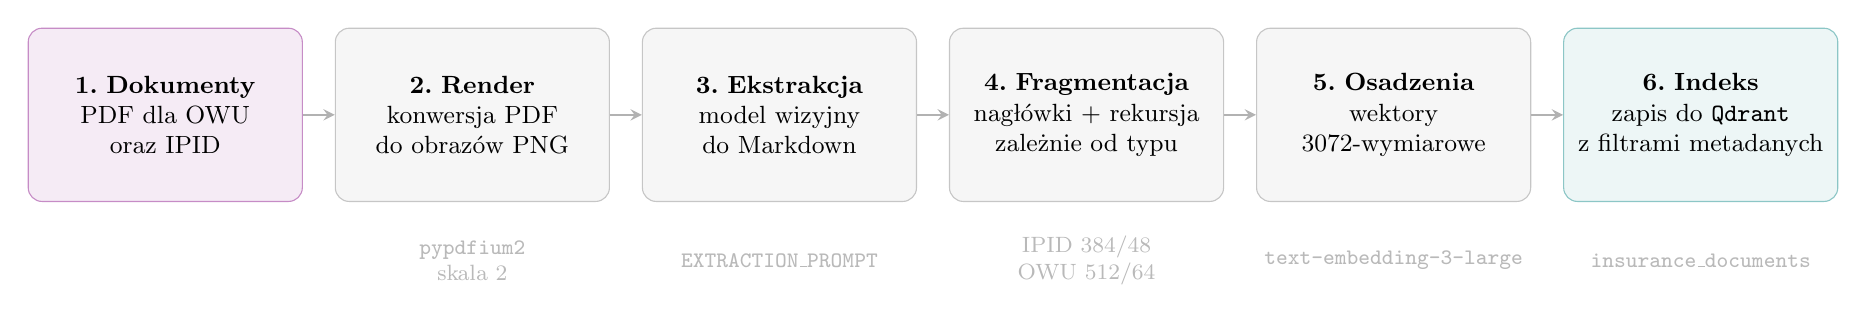
\begin{tikzpicture}[
        flowstep/.style={rectangle, draw, rounded corners=5pt,
          minimum width=3.4cm, minimum height=2.2cm,
          text width=3.2cm, align=center, font=\small,
        fill=gray!7, draw=gray!45, inner sep=4pt},
        arrow/.style={->, >=stealth, thick, draw=gray!60},
        lab/.style={font=\footnotesize, text=gray!55,
        align=center, text width=3.4cm}
      ]
      \node[flowstep, fill=violet!8, draw=violet!45] (pdf) at (0,    0)
      {\textbf{1.~Dokumenty}\\PDF dla OWU\\oraz IPID};
      \node[flowstep] (ocr)  at (3.9,  0)
      {\textbf{2.~Render}\\konwersja PDF\\do obrazów PNG};
      \node[flowstep] (md)   at (7.8,  0)
      {\textbf{3.~Ekstrakcja}\\model wizyjny\\do Markdown};
      \node[flowstep] (ch)   at (11.7, 0)
      {\textbf{4.~Fragmentacja}\\nagłówki + rekursja\\zależnie od typu};
      \node[flowstep] (emb)  at (15.6, 0)
      {\textbf{5.~Osadzenia}\\wektory\\3072-wymiarowe};
      \node[flowstep, fill=teal!7, draw=teal!45] (qd) at (19.5, 0)
      {\textbf{6.~Indeks}\\zapis do \texttt{Qdrant}\\z~filtrami metadanych};
      \foreach \a/\b in {pdf/ocr,ocr/md,md/ch,ch/emb,emb/qd}
      {\draw[arrow] (\a) -- (\b);}
      \node[lab] at (3.9,  -1.85) {\texttt{pypdfium2}\\skala 2};
      \node[lab] at (7.8,  -1.85) {\texttt{EXTRACTION\_PROMPT}};
      \node[lab] at (11.7, -1.85) {IPID 384/48\\OWU 512/64};
      \node[lab] at (15.6, -1.85) {\texttt{text-embedding-3-large}};
      \node[lab] at (19.5, -1.85) {\texttt{insurance\_documents}};
    \end{tikzpicture}
  \end{adjustbox}
  \zrodlo{opracowanie własne}
\end{figure}

\subsection{Ekstrakcja}\label{subsec:ekstrakcja}

Ekstrakcję realizuje klasa \texttt{Extractor} (\texttt{sources/extractor.py}).
Biblioteka \texttt{pypdfium2} renderuje obraz strony (skala 2), który -- po
zakodowaniu jako Base64 PNG -- trafia do modelu wizyjnego wraz z~promptem.
Kontekst międzystronicowy pozwala dołączyć 1024 znaki z~poprzedniej strony, co
zachowuje ciągłość sekcji rozbitych między arkuszami. Wywołanie powtarzane jest
maksymalnie pięciokrotnie z~wykładniczym opóźnieniem. Wynik stanowi plik
Markdown zapisany w~ustalonej strukturze katalogów.

\subsection{Fragmentacja}\label{subsec:fragmentacja}

Fragmentację tekstu wykonuje klasa \texttt{Chuncker}. Dokument dzielony jest
według nagłówków (poziomy 1--3), a~odpowiednie metadane propagowane są do
poszczególnych fragmentów. Większe sekcje podlegają fragmentacji rekurencyjnej
z~wykorzystaniem parametrów właściwych dla danego typu dokumentu
(tabela~\ref{tab:parametry-fragmentacji}).

\begin{table}[H]
  \caption{Parametry fragmentacji}\label{tab:parametry-fragmentacji}
  \centering
  \small
  \begin{tabular}{@{} l c c c @{}}
    \toprule
    \textbf{Typ dokumentu}
    & \textbf{Rozmiar fragmentu}
    & \textbf{Nakładanie}
    & \textbf{Minimum}                     \\
    \midrule
    IPID & 384                        & 48 & 48 \\
    OWU  & 512                        & 64 & 64 \\
    \bottomrule
  \end{tabular}
  \zrodlo{opracowanie własne}
\end{table}

Rozmiar fragmentów dla dokumentów IPID zredukowano ze względu na zwięzłość
formularzy, natomiast dla dokumentów OWU wartości zwiększono w~celu zachowania
kontekstu długich klauzul. Fragmentom przypisywany jest deterministyczny
identyfikator UUIDv5 (na bazie nazwy pliku, nagłówków i~treści).

\subsection{Indeksowanie}\label{subsec:indeksowanie}

Tworzenie indeksu realizuje klasa \texttt{VectorStore}
(\texttt{sources/vectorstore.py}). Inicjalizuje ona kolekcję
\texttt{insurance\_documents} z~miarą cosinusową, indeksem HNSW oraz indeksami
pól (payload). Przed wektoryzacją do treści fragmentu doklejane są metadane:
firma, produkt, kategoria, typ i~ścieżka nagłówków. Zabieg ten poprawia
dopasowanie wektorowe dla pytań uwzględniających ubezpieczyciela. Zapis w~bazie
\texttt{Qdrant} przebiega partiami. Pola strukturalne indeksowane są jako
\textit{keyword}, co gwarantuje stały czas działania filtrów metadanych.

\section{Infrastruktura ewaluacyjna}\label{sec:infrastruktura-ewaluacyjna}

Warstwę ewaluacyjną podzielono na trzy moduły. Komponent \texttt{Runner}
uruchamia architektury i~zapisuje odpowiedzi. \texttt{Evaluator} oblicza
metryki, korzystając z~usługi \texttt{Phoenix}. \texttt{Observer} inicjalizuje
śledzenie \texttt{OpenTelemetry} i~rejestruje przebiegi. Podział ten
uniezależnia generowanie odpowiedzi od oceny (architektury nie uzyskują
sprzężenia zwrotnego z~ewaluacji).

\subsection{Uruchamianie architektur}\label{subsec:uruchamianie-architektur}

Komponent \texttt{Runner} wczytuje pliki CSV z~pytaniami i~generuje iloczyn
kartezjański par pytanie--architektura (540 przebiegów dla 90 pytań). Wykonanie
zrównoleglono w~puli wątków, wykorzystując \texttt{graph.ainvoke}. Wyniki
logowane są w~sposób ciągły do plików JSONL i~CSV, co zapobiega utracie danych.
Pojedynczy rekord zawiera pytanie, wariant architektury, odpowiedź, metryki
wywołań, koszty oraz pełne metadane wykonania.

\subsection{Ocena odpowiedzi}\label{subsec:ocena-odpowiedzi}

Komponent \texttt{Evaluator} implementuje bibliotekę \texttt{phoenix.evals}.
Normalizuje wyniki i~wykonuje weryfikację pod kątem: wierności
(\textit{faithfulness}), zwięzłości (\textit{conciseness}) oraz poprawności
(\textit{correctness}). Trafność dokumentów (\textit{document relevance})
oceniana jest rozdzielnie (dla cytowanych fragmentów), co izoluje analizę
wyszukiwania od syntezy. Klasyfikatory poprawności i~zwięzłości wykorzystują
pięciostopniowe skale rzutowane na wartości numeryczne.

\subsection{Śledzenie przebiegów}\label{subsec:sledzenie-przebiegow}

Komponent \texttt{Observer} konfiguruje usługę \texttt{Phoenix}
(\texttt{auto\_instrument=True}), co zapewnia automatyczne śledzenie wywołań
bibliotek \texttt{LangChain} i~\texttt{OpenAI}. Ponadto zdefiniowano własne
zakresy monitorowania dla przebiegów architektur i~obliczeń metryk.

Tabela~\ref{tab:artefakty-ewaluacji} zestawia artefakty wyjściowe fazy
ewaluacji.

\begin{table}[H]
  \caption{Artefakty ewaluacji}\label{tab:artefakty-ewaluacji}
  \centering
  \small
  \begin{tabularx}{\textwidth}{@{} l L @{}}
    \toprule
    \textbf{Plik}
    & \textbf{Zawartość}                                    \\
    \midrule
    \texttt{runner\_results\_*.jsonl}
    & Strumieniowy zapis pełnych rekordów uruchomień        \\
    \texttt{runner\_results\_*.csv}
    & Spłaszczona tabela wyników wykonawczych               \\
    \texttt{runner\_results\_*.json}
    & Pełny zapis wyników po zakończeniu biegu              \\
    \texttt{runner\_summary\_*.csv}
    & Zbiorcze metryki operacyjne według architektury       \\
    \texttt{overall\_answer\_metrics\_*.csv}
    & Metryki odpowiedzi na poziomie pojedynczego przebiegu \\
    \texttt{overall\_document\_relevance\_*.csv}
    & Ocena trafności cytowanych fragmentów                 \\
    \texttt{overall\_summary\_*.csv}
    & Zbiorcze podsumowanie ewaluacji \texttt{Phoenix}      \\
    \bottomrule
  \end{tabularx}
  \zrodlo{opracowanie własne}
\end{table}

\section{Wybrane zagadnienia inżynieryjne}\label{sec:wybrane-zagadnienia-inzynieryjne}

\subsection{Zarządzanie rozmiarem okna kontekstowego}\label{subsec:kontrola-rozrostu-kontekstu}

W~systemach RAG nadmierny rozrost kontekstu stanowi istotne ograniczenie
techniczne. Moduł rerankera przycina fragmenty do 1000 znaków i~dzieli dane na
partie (limit 12000 tokenów). Selektor dowodów ogranicza kontekst syntezy do
\texttt{evidence\_top\_k} fragmentów. W~architekturze ReAct zamiast pełnej
treści dokumentów logowane są krótkie podsumowania działań narzędzi, co
uniezależnia rozmiar historii iteracji od liczby pobranych fragmentów.

\subsection{Agregacja metadanych wykonania}\label{subsec:spojnosc-metadanych-wykonania}

Metadane wykonania są agregowane przez funkcję
\texttt{merge\_tracking\_metadata}. Sumuje ona liczniki narzędzi, tokenów
i~kosztów przy jednoczesnym zachowaniu lokalnych zmiennych sterujących.
Mechanizm ten znajduje zastosowanie w~architekturze hierarchicznej oraz
w~funkcji \texttt{retrieve\_multi}, gdzie pojedyncze narzędzie wywoływane jest
wielokrotnie w~ramach jednego węzła.

\subsection{Obsługa niepoprawnych wyjść modeli}\label{subsec:odpornosc-na-niepoprawne-wyjscia-modeli}

Komponenty zależne od formatu JSON wyposażono w~ścieżki awaryjne. Parser zwraca
metadane neutralne, rewriter powiela zapytanie bazowe, planer stosuje wariant
deterministyczny, a~dekompozytor nie dzieli pytania. Architektura ReAct loguje
nierozpoznaną akcję jako obserwację. Błędy są rejestrowane, jednak system
gwarantuje zwrócenie kontrolowanego wyniku końcowego.

\subsection{Strategia wielojęzycznych promptów}\label{subsec:dwujezyczny-charakter-promptow}

Instrukcje systemowe sformułowano w~języku angielskim (z~uwagi na zwięzłość
i~zgodność z~formatami danych), natomiast pytania, dokumenty i~odpowiedzi
pozostają polskojęzyczne. Prompty odpowiedziowe wymuszają generowanie tekstu
w~języku polskim oraz zakazują korzystania z~wiedzy zewnętrznej.

\subsection{Stabilność identyfikatorów fragmentów}\label{subsec:idempotencja-indeksowania}

Identyfikatory fragmentów generowane są deterministycznie (algorytm UUIDv5) na
podstawie metadanych i~treści. Gwarantuje to identyczność kluczy w~bazie
\texttt{Qdrant} przy kolejnych uruchomieniach potoku dla niezmienionego
korpusu, co pozwala na przyrostową aktualizację i~porównywanie wyników.

\subsection{Izolacja warstwy ewaluacyjnej}\label{subsec:oddzielenie-ewaluacji-od-wykonania}

Ewaluator operuje wyłącznie na utrwalonych artefaktach. Architektury nie
modyfikują odpowiedzi na podstawie wyników z~\texttt{Phoenix}. Separacja ta
zapewnia odtwarzalność procesu: surowe pliki wynikowe mogą być poddawane
ponownej ocenie (z~użyciem innych ewaluatorów lub rubryk) bez konieczności
powtarzania przebiegów.